

Restricciones importantes que incorporamos:

Para atleta, entrenador y arbitro hemos decidido que sean entidades hijas de Persona, ya que todas comparten que deben tener los mismo datos básicos

Realizamos agregación en la parte de medallero ya que necesitamos involucrar qué \textbf{atletas} ganaron medallas, es decir, cuáles son \textbf{ganadores} y de ahí contabilizar las medallas en los \textbf{países}. 

En la relación Ser Ganador hemos decidido guardar el Número de medallas para los países, esto para contabilizar al final cuántos atletas de medalla de oro (plata, o bronce según el caso) tiene determinado país y asignar el Medallero.

Localidad que dependerá de que haya una disciplina en el lugar, por ello, Localidad también guardará el nombre de la Disciplina que impartirá.

\begin{center}
    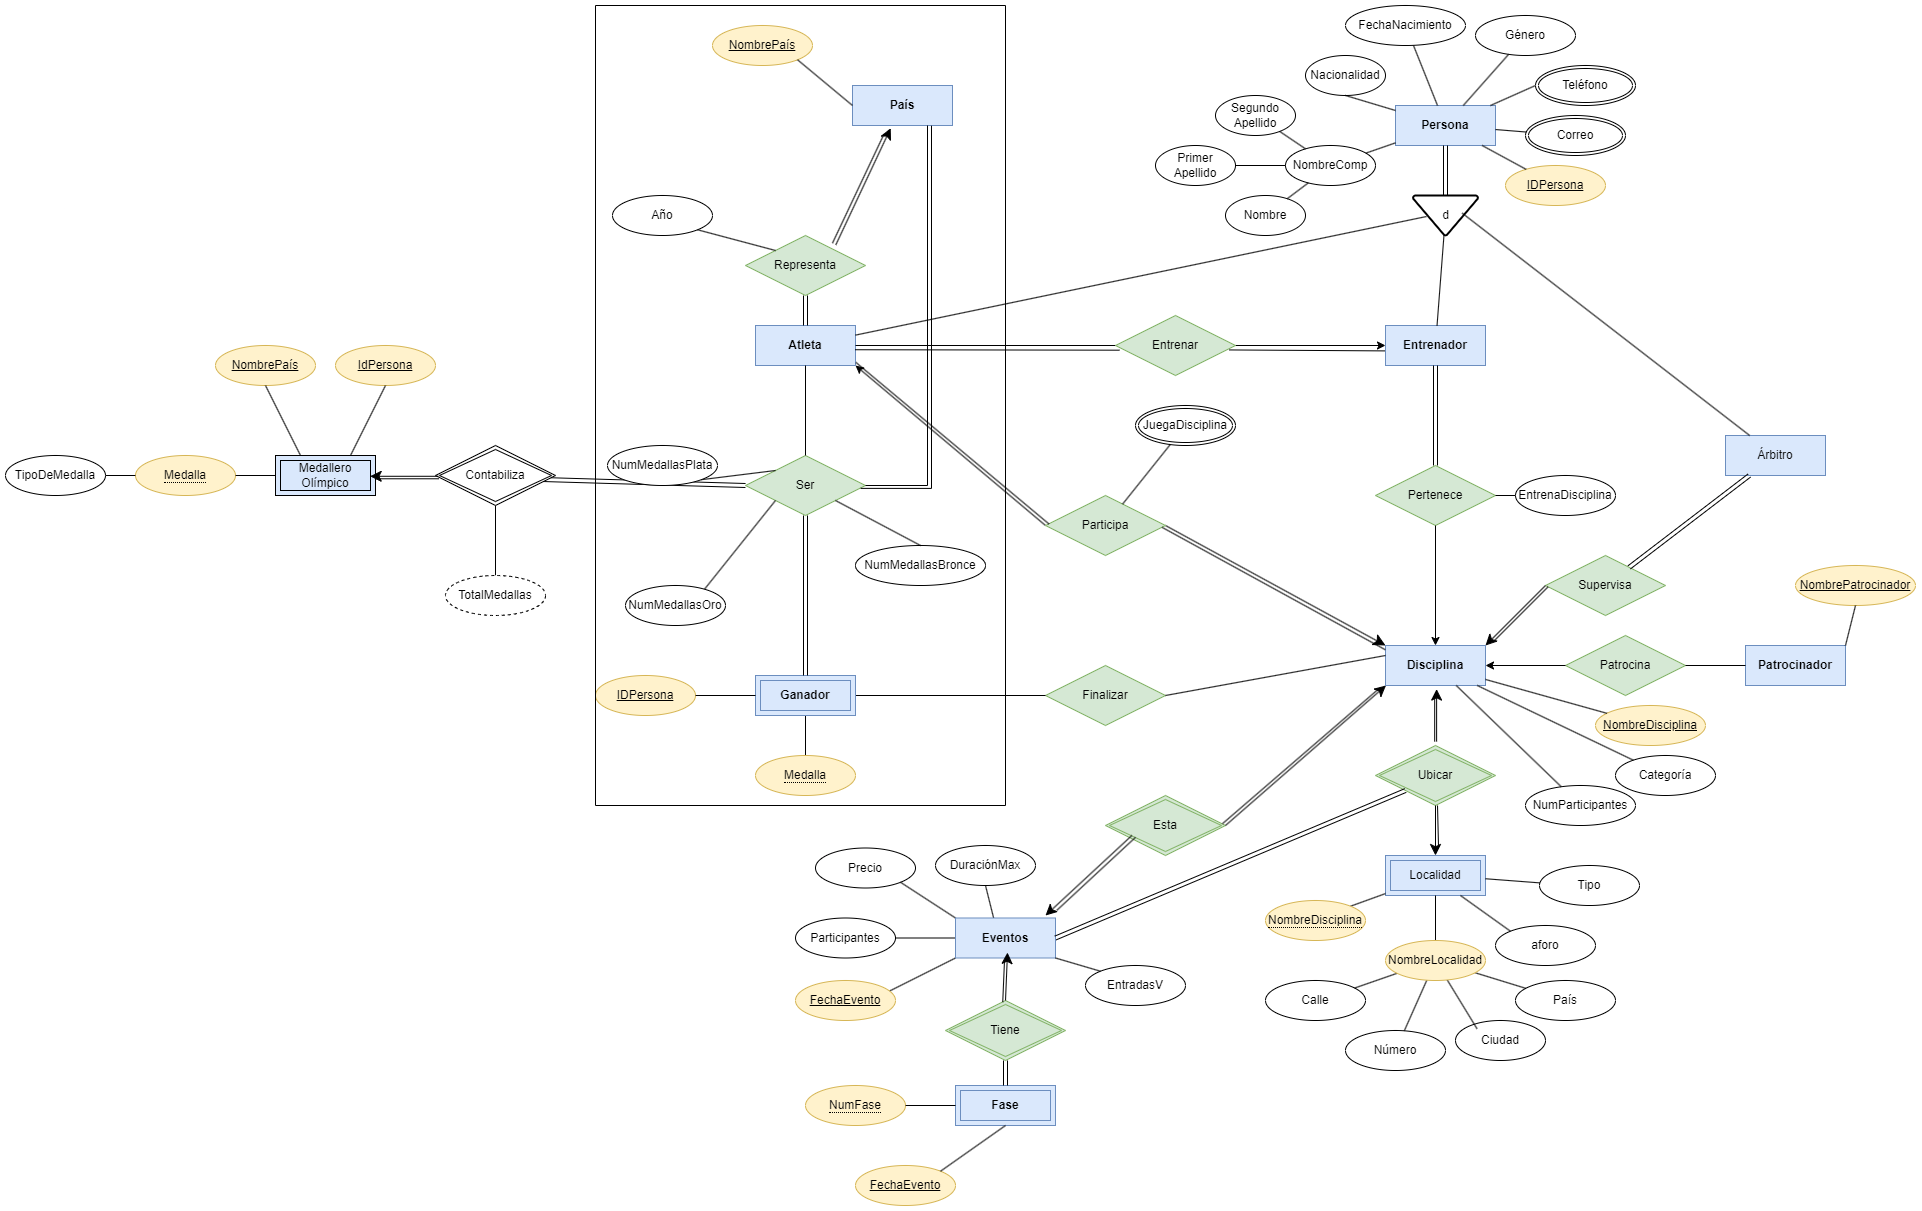
\includegraphics[width=17cm]{resources/DiagramaOlimpiadas.png}
\end{center}


